%%%%%%%%%%%%%%%%%%%%%%%%%%%%%%%%%%%%%%%%%%%%%%%%%%%%%%%%%%%%%%%%%%%%
%% I, the copyright holder of this work, release this work into the
%% public domain. This applies worldwide. In some countries this may
%% not be legally possible; if so: I grant anyone the right to use
%% this work for any purpose, without any conditions, unless such
%% conditions are required by law.
%%%%%%%%%%%%%%%%%%%%%%%%%%%%%%%%%%%%%%%%%%%%%%%%%%%%%%%%%%%%%%%%%%%%

\documentclass[
  digital,     %% The `digital` option enables the default options for the
               %% digital version of a document. Replace with `printed`
               %% to enable the default options for the printed version
               %% of a document.
%%  color,       %% Uncomment these lines (by removing the %% at the
%%               %% beginning) to use color in the printed version of your
%%               %% document
  oneside,     %% The `oneside` option enables one-sided typesetting,
               %% which is preferred if you are only going to submit a
               %% digital version of your thesis. Replace with `twoside`
               %% for double-sided typesetting if you are planning to
               %% also print your thesis. For double-sided typesetting,
               %% use at least 120 g/m² paper to prevent show-through.
  nosansbold,  %% The `nosansbold` option prevents the use of the
               %% sans-serif type face for bold text. Replace with
               %% `sansbold` to use sans-serif type face for bold text.
  nocolorbold, %% The `nocolorbold` option disables the usage of the
               %% blue color for bold text, instead using black. Replace
               %% with `colorbold` to use blue for bold text.
  lof,         %% The `lof` option prints the List of Figures. Replace
               %% with `nolof` to hide the List of Figures.
  lot,         %% The `lot` option prints the List of Tables. Replace
               %% with `nolot` to hide the List of Tables.
]{fithesis4}
%% The following section sets up the locales used in the thesis.
\usepackage[resetfonts]{cmap} %% We need to load the T2A font encoding
\usepackage[T1,T2A]{fontenc}  %% to use the Cyrillic fonts with Russian texts.
\usepackage[
  main=english, %% By using `czech` or `slovak` as the main locale
                %% instead of `english`, you can typeset the thesis
                %% in either Czech or Slovak, respectively.
  english, german, russian, czech, slovak %% The additional keys allow
]{babel}        %% foreign texts to be typeset as follows:
%%
%%   \begin{otherlanguage}{german}  ... \end{otherlanguage}
%%   \begin{otherlanguage}{russian} ... \end{otherlanguage}
%%   \begin{otherlanguage}{czech}   ... \end{otherlanguage}
%%   \begin{otherlanguage}{slovak}  ... \end{otherlanguage}
%%
%% For non-Latin scripts, it may be necessary to load additional
%% fonts:
\usepackage{paratype}
\def\textrussian#1{{\usefont{T2A}{PTSerif-TLF}{m}{rm}#1}}
%%
%% The following section sets up the metadata of the thesis.
\thesissetup{
    date        = \the\year/\the\month/\the\day,
    university  = mu,
    faculty     = fi,
    type        = bc,
    department  = Department of Computer Systems and Communications,
    author      = Tomáš Zobač,
    gender      = m,
    advisor     = {RNDr. Rudolf Wittner},
    title       = {Implementation of provenance chains traversal},
    TeXtitle    = {Implementation of provenance chains traversal},
    keywords    = {Java, provenance, SOBHA, ÚVT},
    TeXkeywords = {Java, provenance, SOBHA, ÚVT},
    abstract    = {%
      Provenance is a standardized information type that documents the history of an object. It can hold information, such as the origin of an object or previous actions performed on it. This information can be serialized into one of the many supported file formats (e.g., PROVN, XML). These files can then be interconnected, resulting in the creation of a provenance chain. This thesis aims to implement a library for traversing said provenance chains, retrieving information about the precursors or successors of an entity represented in one of the files in the current chain, and optionally retrieving the type of actions performed on the object by the retrieved precursors/successors. The implementation will simulate the operational environment by providing a command-line user interface from where the user can call the mentioned actions on a set of prefactured simulation files. The implementation will follow a W3C PROV-DM standard for provenance notation, and the simulation files will be of a PROVN serialization of provenance data. Additionally to the traversing operations, it will also implement the generation of a provenance metadata to make the simulation of a traversal possible.
    },
    thanks      = {%
      TODO
    },
    bib         = example.bib,
    %% Remove the following line to use the JVS 2018 faculty logo.
    facultyLogo = fithesis-fi,
}
\usepackage{makeidx}      %% The `makeidx` package contains
\makeindex                %% helper commands for index typesetting.
%% These additional packages are used within the document:
\usepackage{paralist} %% Compact list environments
\usepackage{amsmath}  %% Mathematics
\usepackage{amsthm}
\usepackage{amsfonts}
\usepackage{url}      %% Hyperlinks
\usepackage{markdown} %% Lightweight markup
\usepackage{listings} %% Source code highlighting
\lstset{
  basicstyle      = \ttfamily,
  identifierstyle = \color{black},
  keywordstyle    = \color{blue},
  keywordstyle    = {[2]\color{cyan}},
  keywordstyle    = {[3]\color{olive}},
  stringstyle     = \color{teal},
  commentstyle    = \itshape\color{magenta},
  breaklines      = true,
}
\usepackage{floatrow} %% Putting captions above tables
\floatsetup[table]{capposition=top}
\usepackage[babel]{csquotes} %% Context-sensitive quotation marks
\begin{document}
%% The \chapter* command can be used to produce unnumbered chapters:
\chapter*{Introduction}
%% Unlike \chapter, \chapter* does not update the headings and does not
%% enter the chapter to the table of contents. I we want correct
%% headings and a table of contents entry, we must add them manually:
\markright{\textsc{Introduction}}
\addcontentsline{toc}{chapter}{Introduction}

Theses are rumoured to be \enquote{the capstones of education}, so
I decided to write one of my own. If all goes well, I will soon
have a diploma under my belt. Wish me luck!


\chapter{Provenance}
\shorthandoff{-}
Provenance refers to the collective information about the history or origin of something, especially its ownership or location history. It is often used in contexts where it is essential to trace the history of an object, idea, or practice to establish its authenticity, origin, and how it was handled through time. For example, in literature, provenance can relate to the history of a manuscript or a book. Knowing who owned a rare manuscript, where it was kept, and how it was passed down through generations can shed light on its historical importance and authenticity.

In the digital realm, provenance refers to the documentation of the history of data, including its origins, processing, and storage. This is particularly significant, especially in fields such as scientific research, where tracking the origin and modifications of data ensures its reliability and reproducibility. Provenance is the term used to describe all the information and data referred to in the abovementioned examples. It is the collective name given to this type of data.
\shorthandon{-}

\section{PROV-DM}
\shorthandoff{-}
In order to represent the provenance in a format that can be easily shared and processed, the W3C PROV-DM (Provenance Data Model) standard was created. The PROV-DM is structured as a directed graph, representing provenance through nodes and edges. 

Nodes in this graph are defined as Entities, Activities, and Agents, each playing a distinct role. Entities refer to physical, digital, or other objects central to or associated with the provenance. Activities encompass actions and processes conducted on or with these entities. Agents are the nodes that perform activities, effectively creating or influencing entities and activities.

The edges in this graph refer to the relations between these nodes. Examples include 'wasDerivedFrom,' 'wasGeneratedBy,' and 'used,' which help map out the model's interactions.

Moreover, the PROV-DM standard includes a concept known as 'bundles.' These are used to group sets of provenance information, enabling the encapsulation of various model elements. This addition allows for a more nuanced and organized representation of provenance data, enhancing the model's capability to be easily shared and processed.
\shorthandon{-}

\subsection{PROV-N}
\shorthandoff{-}
PROV-N is a vital component of the W3C PROV suite, designed to model provenance and represent it in a human-readable textual format. This format organizes provenance information into three main sections: namespace declarations, statements, and bundles. 

Namespace declarations simplify the identification of entities, activities, and agents by providing a shorthand prefix to a longer namespace URI. For instance, an entity might be identified using a QualifiedName, such as "ns\_surgery:sampleConnector." This notation combines a namespace URI, a readable prefix, and the local part, ensuring that each component is uniquely identified and easily referenced. Namespaces are declared as follows:

\begin{verbatim}

prefix ns_surgery <ns_surgery_URI>
prefix ns_pathology <ns_pathology_URI>

\end{verbatim}

Statements in PROV-N describe the various provenance elements and their relationships. They can range from simple declarations to complex narratives explaining how different entities interact. For example, an entity might be described as "entity(ns\_surgery:sampleConnector)" with attributes detailing its characteristics:

\begin{verbatim}

entity(ns_surgery:sampleConnector, [
    prov:type='cpm:forwardConnector', 
    cpm:receiverBundleId='ns_pathology:02_scanning.provn', 
    cpm:receiverServiceUri="#URI#"
    ])
    
\end{verbatim}

Bundles, as mentioned in "1.1", allow for grouping related provenance information. This organization aids in managing complex provenance scenarios, where it is crucial to encapsulate different aspects of the provenance in distinct, manageable units. The finished document, with declared namespaces and a bundle encapsulating its statements, could look like this example:

\begin{verbatim}

document
  prefix ns_surgery <ns_surgery_URI>

  bundle ns_surgery:01_sample_acquisition.provn
    prefix ns_surgery <ns_surgery_URI>
    prefix ns_pathology <ns_pathology_URI>
    prefix cpm <cpm_URI>

    entity(ns_surgery:sampleConnector,[
        prov:type='cpm:senderConnector',
        cpm:receiverBundleId='ns_pathology:02_scanning.provn',
        cpm:receiverServiceUri="#URI#"
    ])
  endBundle
endDocument

\end{verbatim}

The flexibility of PROV-N is enhanced through its extension support. Users can add custom attributes and define new statements, tailoring the format to specific needs. This adaptability makes PROV-N an ideal choice for various applications, from academic research to industry practices.
\shorthandon{-}

\section{Provenance chain} \label{s-provchain}
\shorthandoff{-}
In the context of W3C PROV modeling, the provenance chain is a sequence of interconnected bundles, each encapsulating a graph with a semi-defined structure. Each bundle in the chain contains a directed graph composed of three main types of entities designed to establish connections within and between bundles.

At the core of this structure are two entry point entities: backwardConnector and forwardConnector. The backwardConnector links to a forwardConnector in the preceding bundle, creating a backward traversal path. Conversely, the forwardConnector establishes a forward link to a backwardConnector in the subsequent bundle. This arrangement ensures a continuous and traceable path through the chain of bundles, allowing for easy navigation.

Additionally, each bundle includes a currentConnector entity. This entity is pivotal in identifying the current bundle within the chain, providing a reference point for the contained provenance information.

While the example given simplifies the structure, it is important to note that, in practice, a single bundle can contain multiple connectors of each type. This multiplicity allows for connections to more than one bundle on either side of the traversal path, thereby accommodating complex provenance scenarios. The ability to link multiple bundles through various connectors enhances the flexibility and depth of the provenance chain, enabling a more detailed and comprehensive representation of the provenance.

With its series of linked bundles and partially predefined configuration, this chain structure offers a robust framework for documenting, tracking, and analyzing the provenance.

\begin{figure}[htbp]
  \begin{center}
    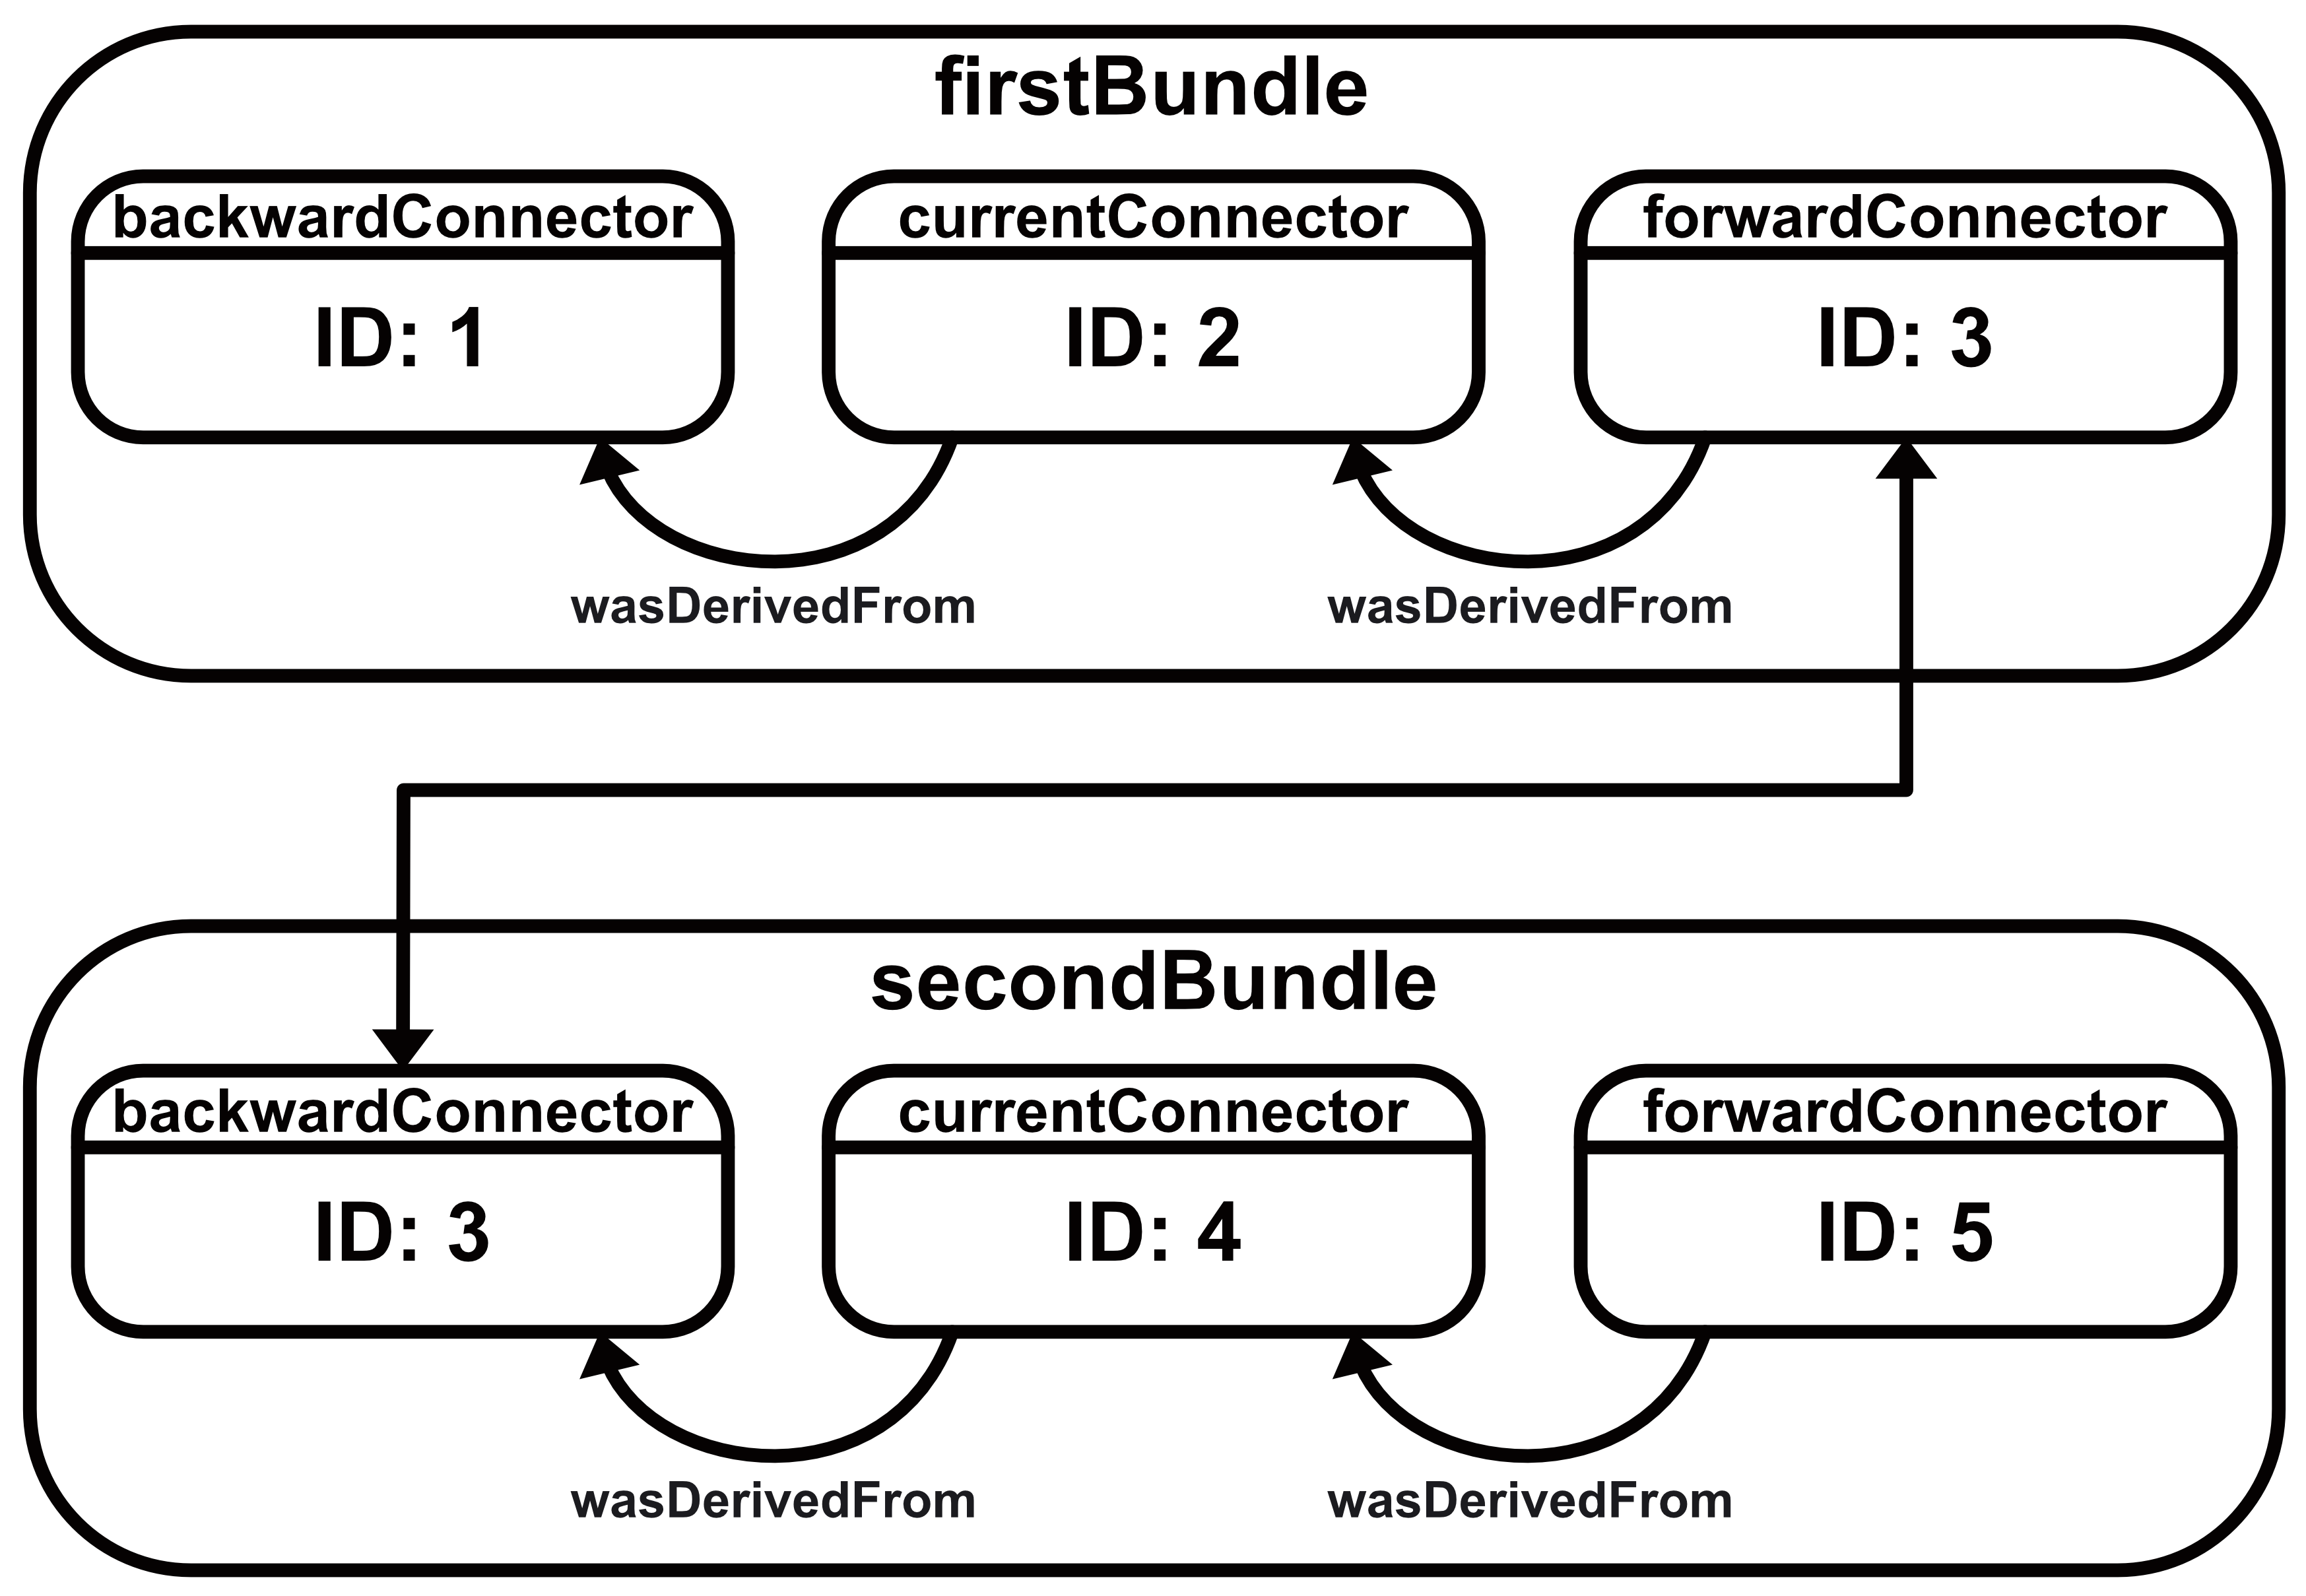
\includegraphics[width=12.5cm]{fithesis/images/bundleconnection.png}
  \end{center}
  \caption{Connection of two provenance bundles}
  \label{fig:bundleconnection}
\end{figure}
\shorthandon{-}
TODO

\chapter{Design}
\shorthandoff{-}
This chapter delves into the architecture and logic of the library, which was developed as an implementation part of this thesis. The chapter has three main objectives. Firstly, it aims to provide a clear and concise overview of the structure of the library and its components, including their respective roles in the library's lifecycle. Secondly, it discusses the simulated environment of a real-world distribution and how it works. Finally, it describes the primary logic used for traversing a provenance chain. It is crucial to explain these specific details to understand the technical implementation described in the succeeding chapter. 
\shorthandon{-}
\section{Structure}
\shorthandoff{-}
At its core, the implementation is designed as a modular, multi-component library. Each component serves a distinct role but contributes to cohesive functionality. This modular approach facilitates easy maintenance and scalability. Central to this structure is a layered architecture, segregating the library operations into distinct layers - data retrieval, processing, and presentation. 
The data retrieval layer is responsible for acquiring the PROV-N data, depending on the type of storage, and deserializing it into a unified type. 
The processing layer handles the traversal of the provenance chain as well as the traversal of the directed graph inside each PROV-N document. It is also responsible for evaluating the documents' integrity and retrieving the relevant provenance data.
Finally, the presentation layer provides the interface for user interaction, enabling command inputs and displaying results on the command line.
\shorthandon{-}

\subsection{Components}
\shorthandoff{-}
The library's components are separated into four main parts.
\begin{enumerate}
    \item \textbf{Main UI:}
        This component is tasked with the preparation of resources for the library and providing a user interface on the command line, where the user can input commands and view the results of the entered queries. The user interface also provides quality-of-life functions, such as command auto-completion, command history, or in-command query history.
    \item \textbf{Configuration:}
        This set of components retrieves data from a configuration JSON file and passes it to the library.
    \item \textbf{Tools:}
        This set of components serves as a toolset for the library. The first set of tools retrieves and deserializes PROV-N documents depending on their storage type. It currently supports retrieving files saved locally in the file system and remotely in GitLab repositories. 
        The second set of tools is used to resolve persistent identifiers stored in the relevant navigation table.
        The third is used for retrieving hash values from the corresponding meta-provenance, and the last is used for hash creation.
    \item \textbf{Main logic:}
        This last set of components handles the data processing. It traverses the provenance chain and retrieves the user-specified data. It also assures the correctness of the traversed chain by evaluating the integrity of the document using its hash values stored in the corresponding meta-provenance and comparing it to new hash values created using the last set of tools.
\end{enumerate}
\shorthandon{-}

\section{Simulation}
\shorthandoff{-}
For the implementation to simulate a real-world environment, some regulations had to be established specifically for this thesis. The PROV-N serialization will be the only one used in this thesis. The PROV-N documents used in the implementation were generated and provided by the thesis supervisor using the "cite thesis". These documents follow a predefined structure and naming rules described in the standard currently being developed by the supervisor and his colleagues. The implementation will also include a package for generating meta-provenance, which will be used for the provided documents. Lastly, the resolution of the persistent identifiers will be done with an in-memory navigation table created during the library's initialization process containing all of the provided documents.
\shorthandon{-}

\section{Algorithm}
\shorthandoff{-}
As mentioned before in section \ref{s-provchain}, the main structure of a bundle consists of three Entities with predefined connector types connected by the wasDerivedFrom statements. As an example of the traversal, assume the algorithm has already traversed one bundle and is now entering a succeeding one with its graph's structure, as shown in Figure.

\begin{figure}[htbp]
  \begin{center}
    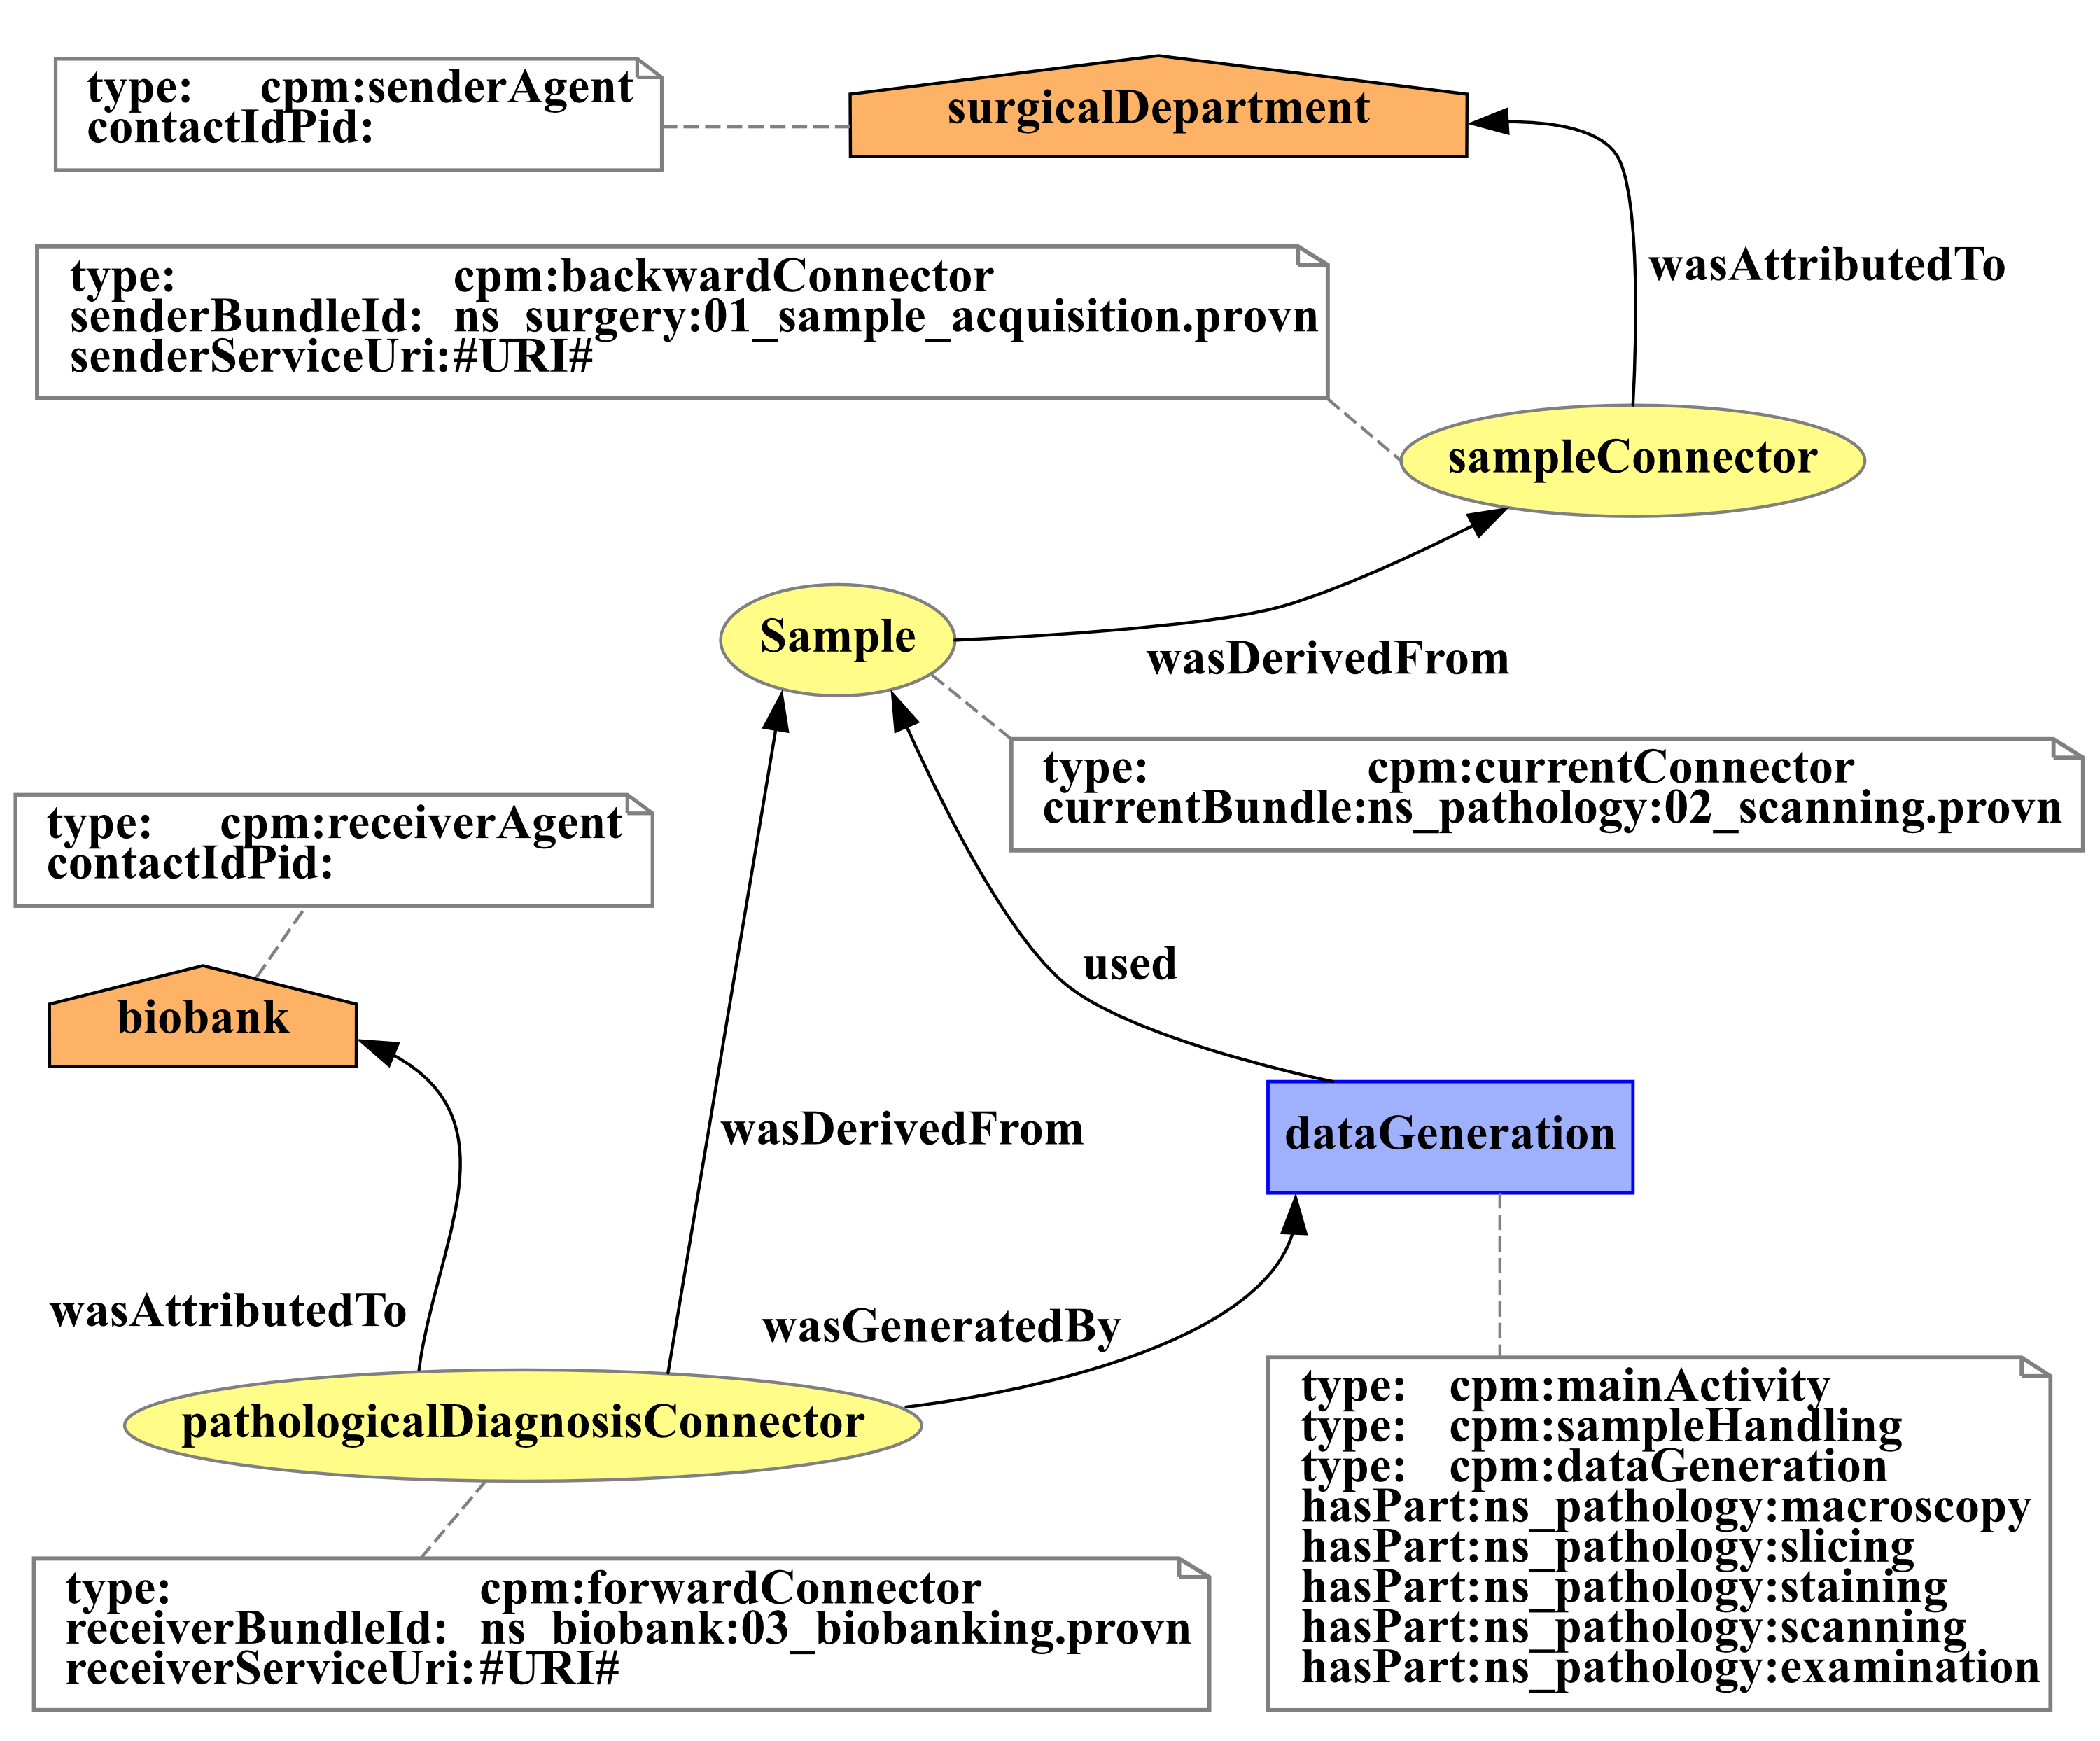
\includegraphics[width=9cm]{fithesis/images/examplebigger.png}
  \end{center}
  \caption{Excerpt from a PROV-N document}
  \label{fig:bundleexample}
\end{figure}
\shorthandon{-}

Considering the algorithm arrived from the bundle 01\_sample\_acquisition,
the next step is to use a wasDerivedFrom statement where the
backwardConnector is in the role of a used Entity.

\begin{figure}[htbp]
  \begin{center}
    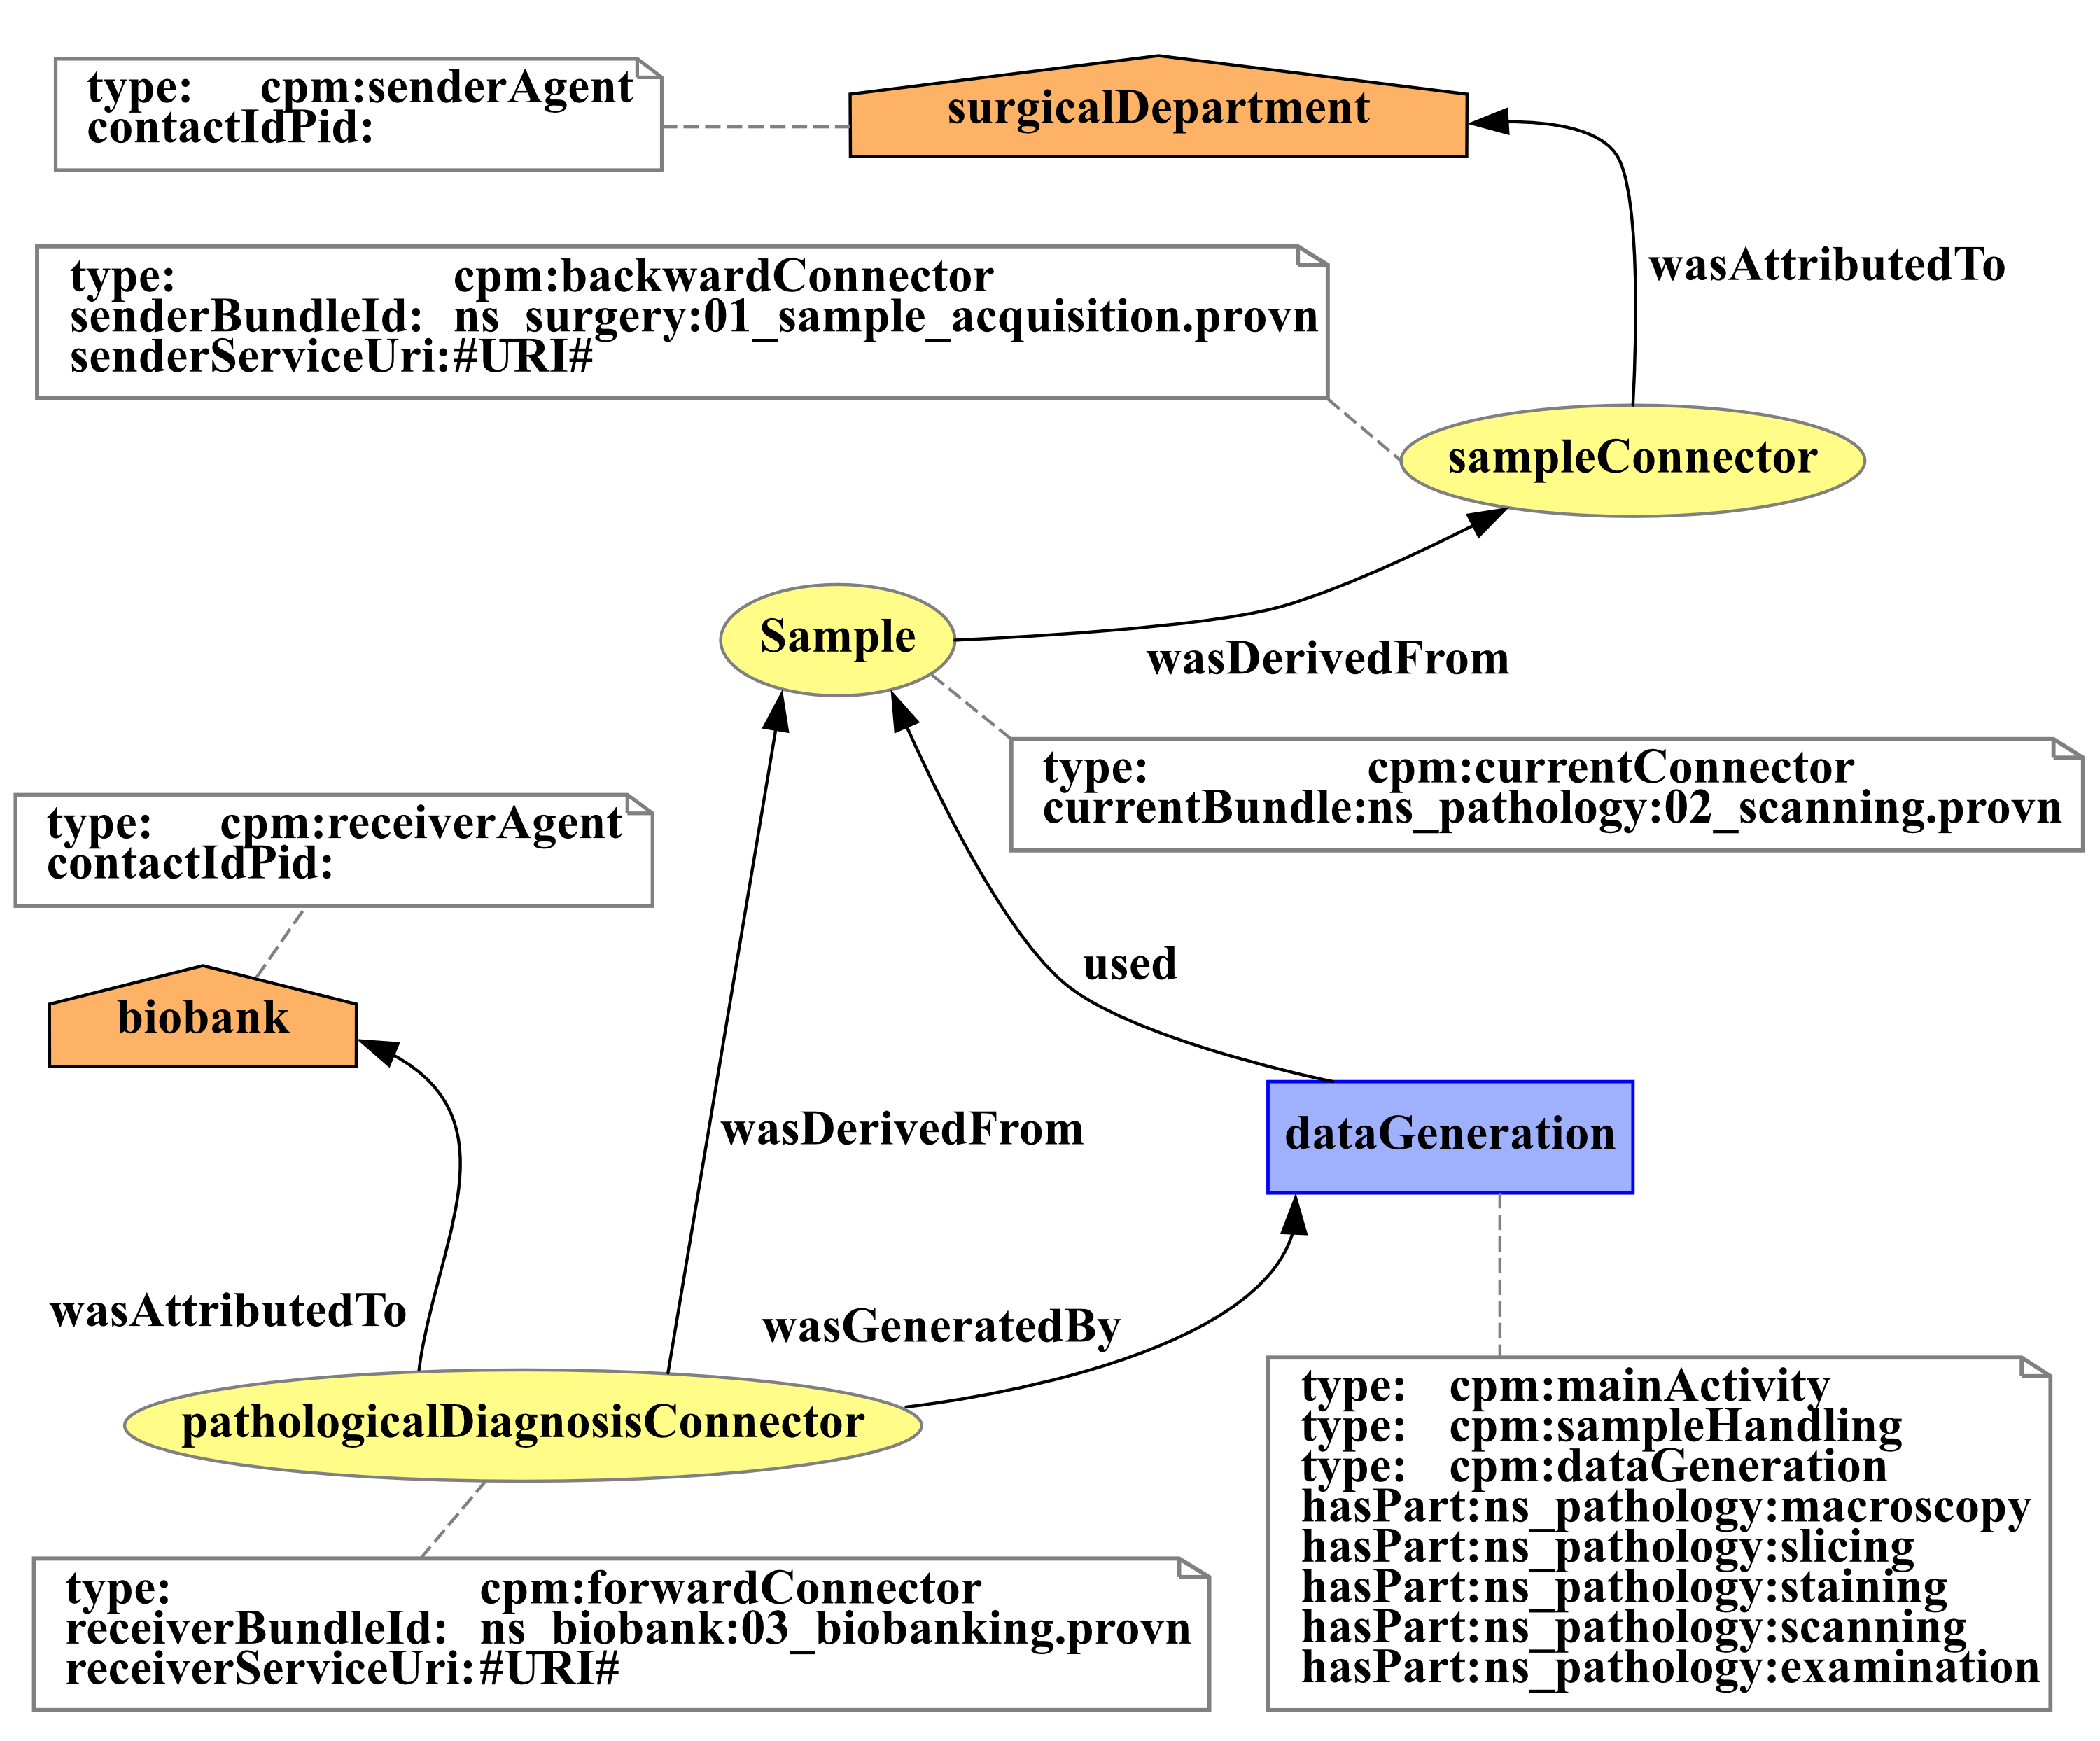
\includegraphics[width=9cm]{fithesis/images/examplebigger.png}
  \end{center}
  \caption{Excerpt from a PROV-N document}
  \label{fig:bundleexample2}
\end{figure}

After moving to the currentConnector, the algorithm again finds a wasDerivedFrom statement where the currentConnector is in the role of a used Entity, and the forwardConnector is in the role of a generated Entity.

\begin{figure}[htbp]
  \begin{center}
    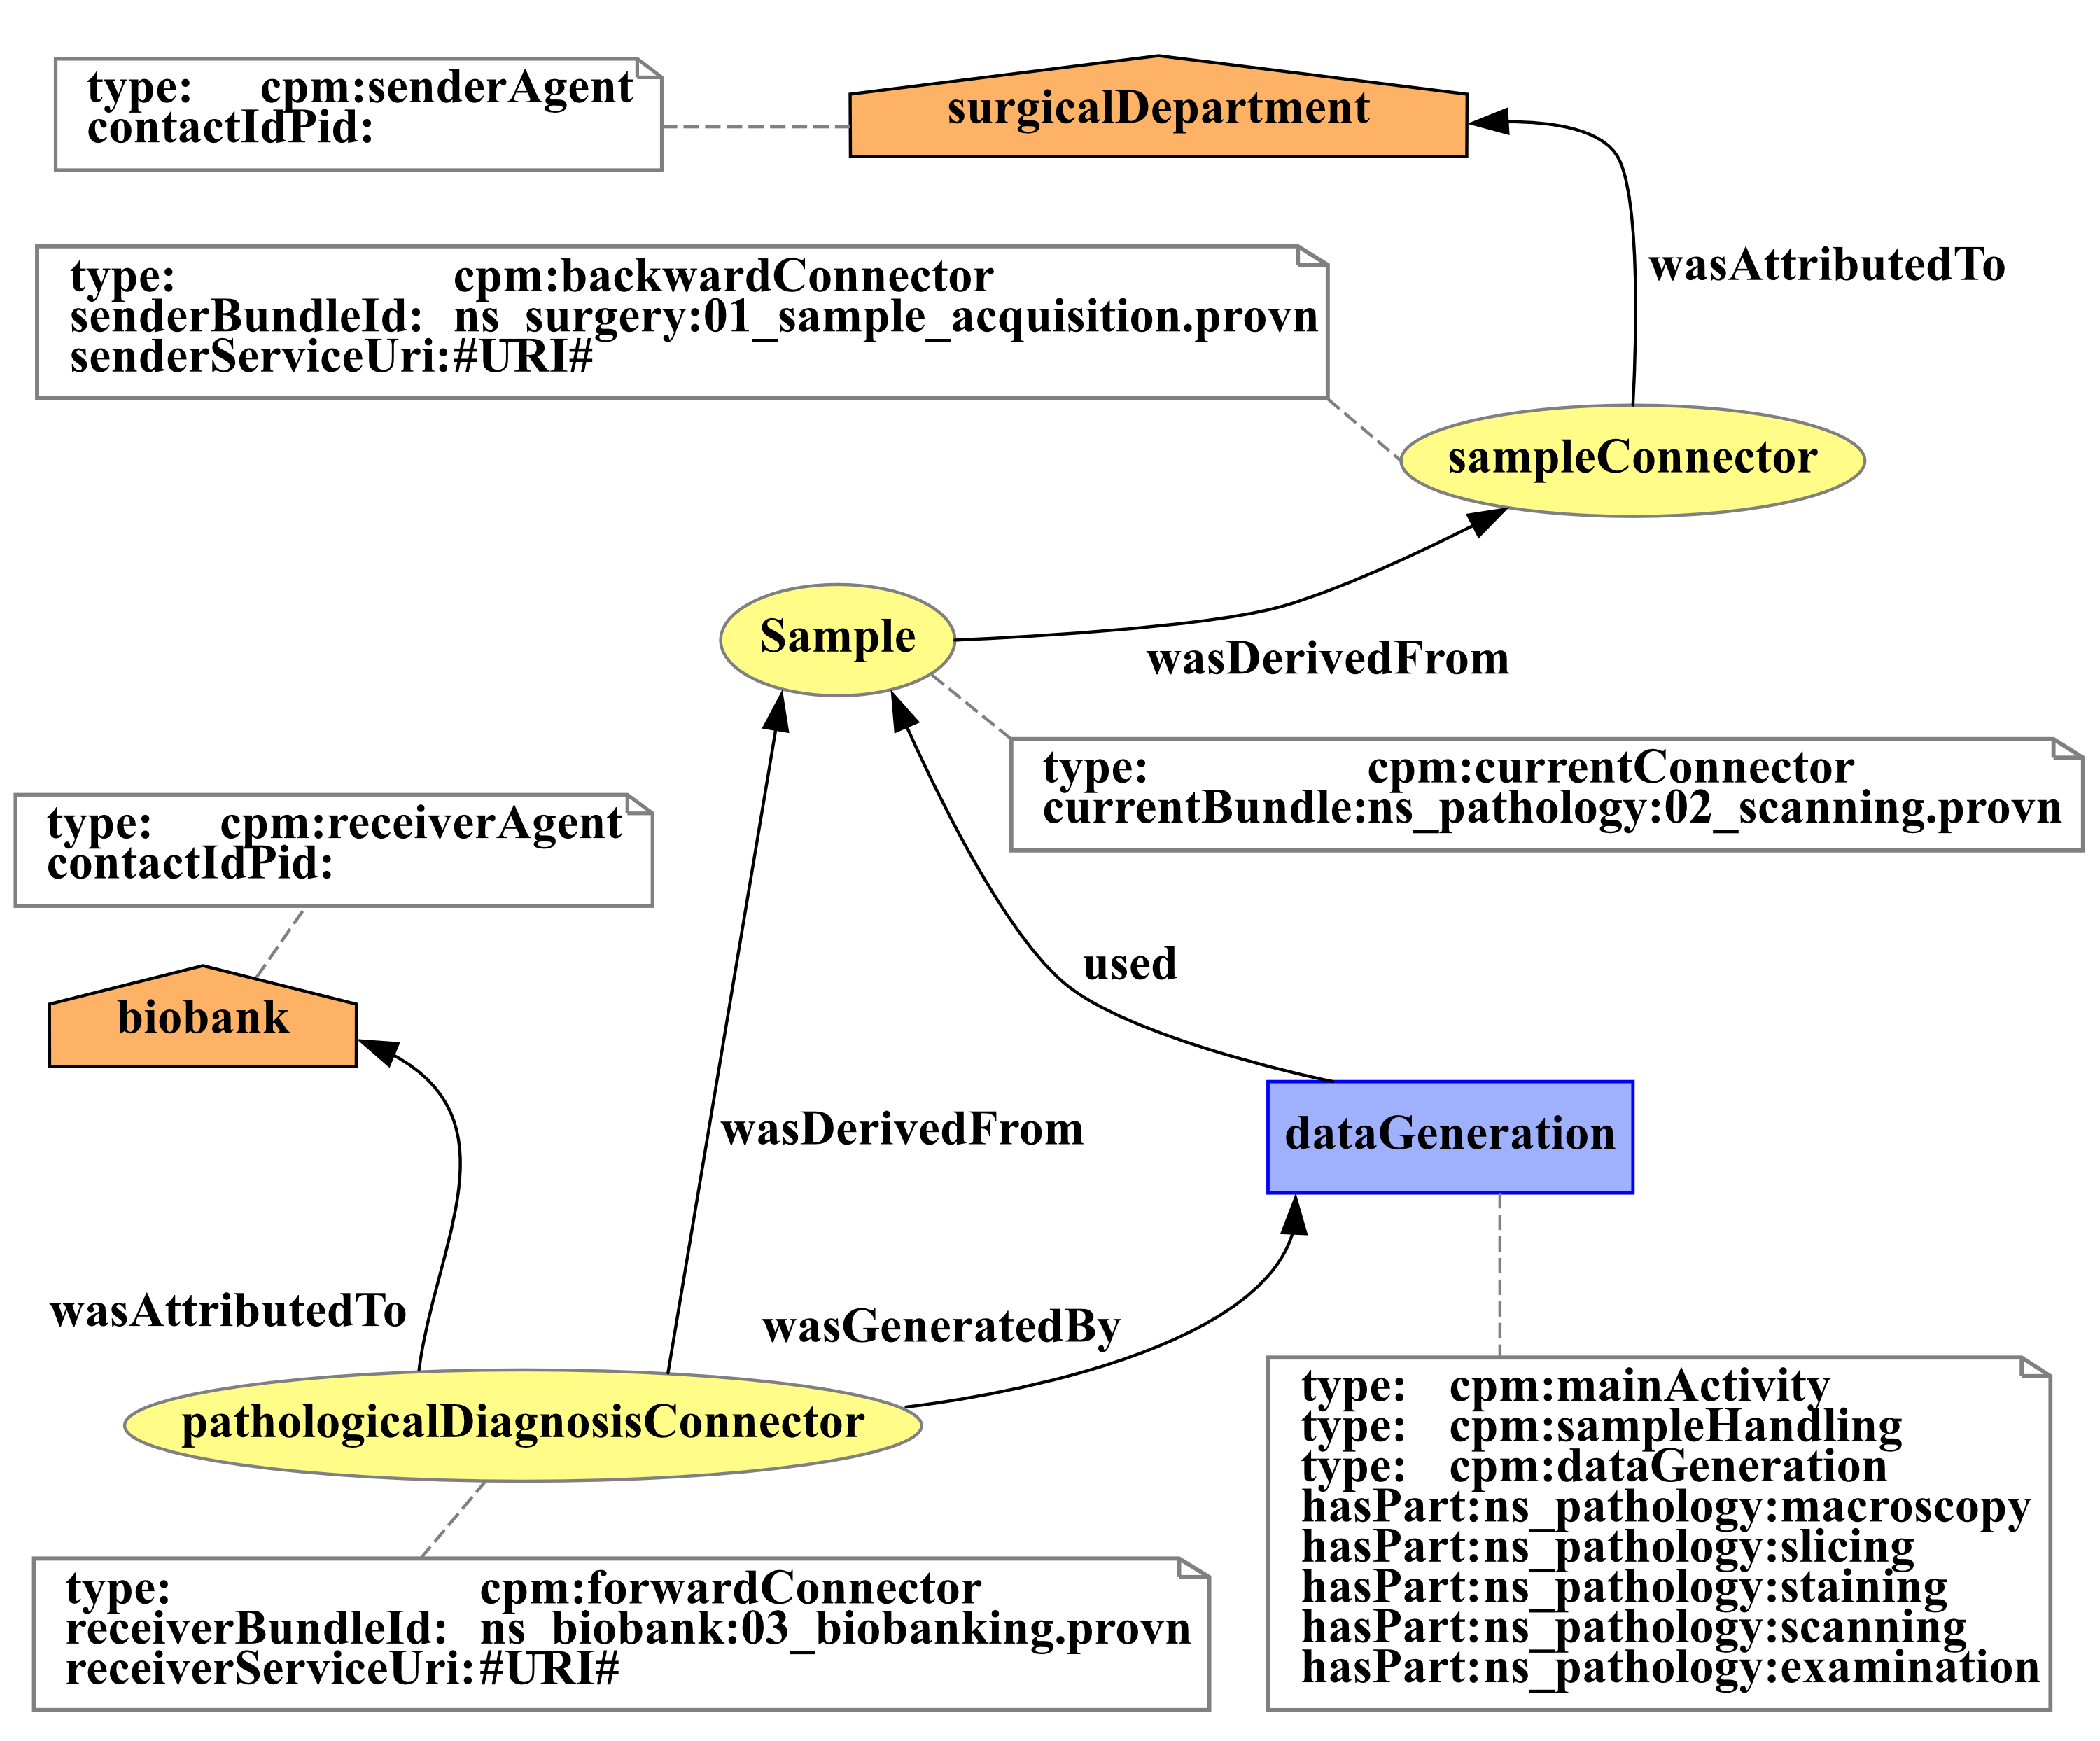
\includegraphics[width=9cm]{fithesis/images/examplebigger.png}
  \end{center}
  \caption{Excerpt from a PROV-N document}
  \label{fig:bundleexample3}
\end{figure}

After reaching the end of the bundle's graph, the algorithm can enter another bundle by looking into the current forwardConnector's attributes, retrieving the succeeding bundle's identifier (Figure 1.1), and executing the whole process again.

\begin{figure}[htbp]
  \begin{center}
    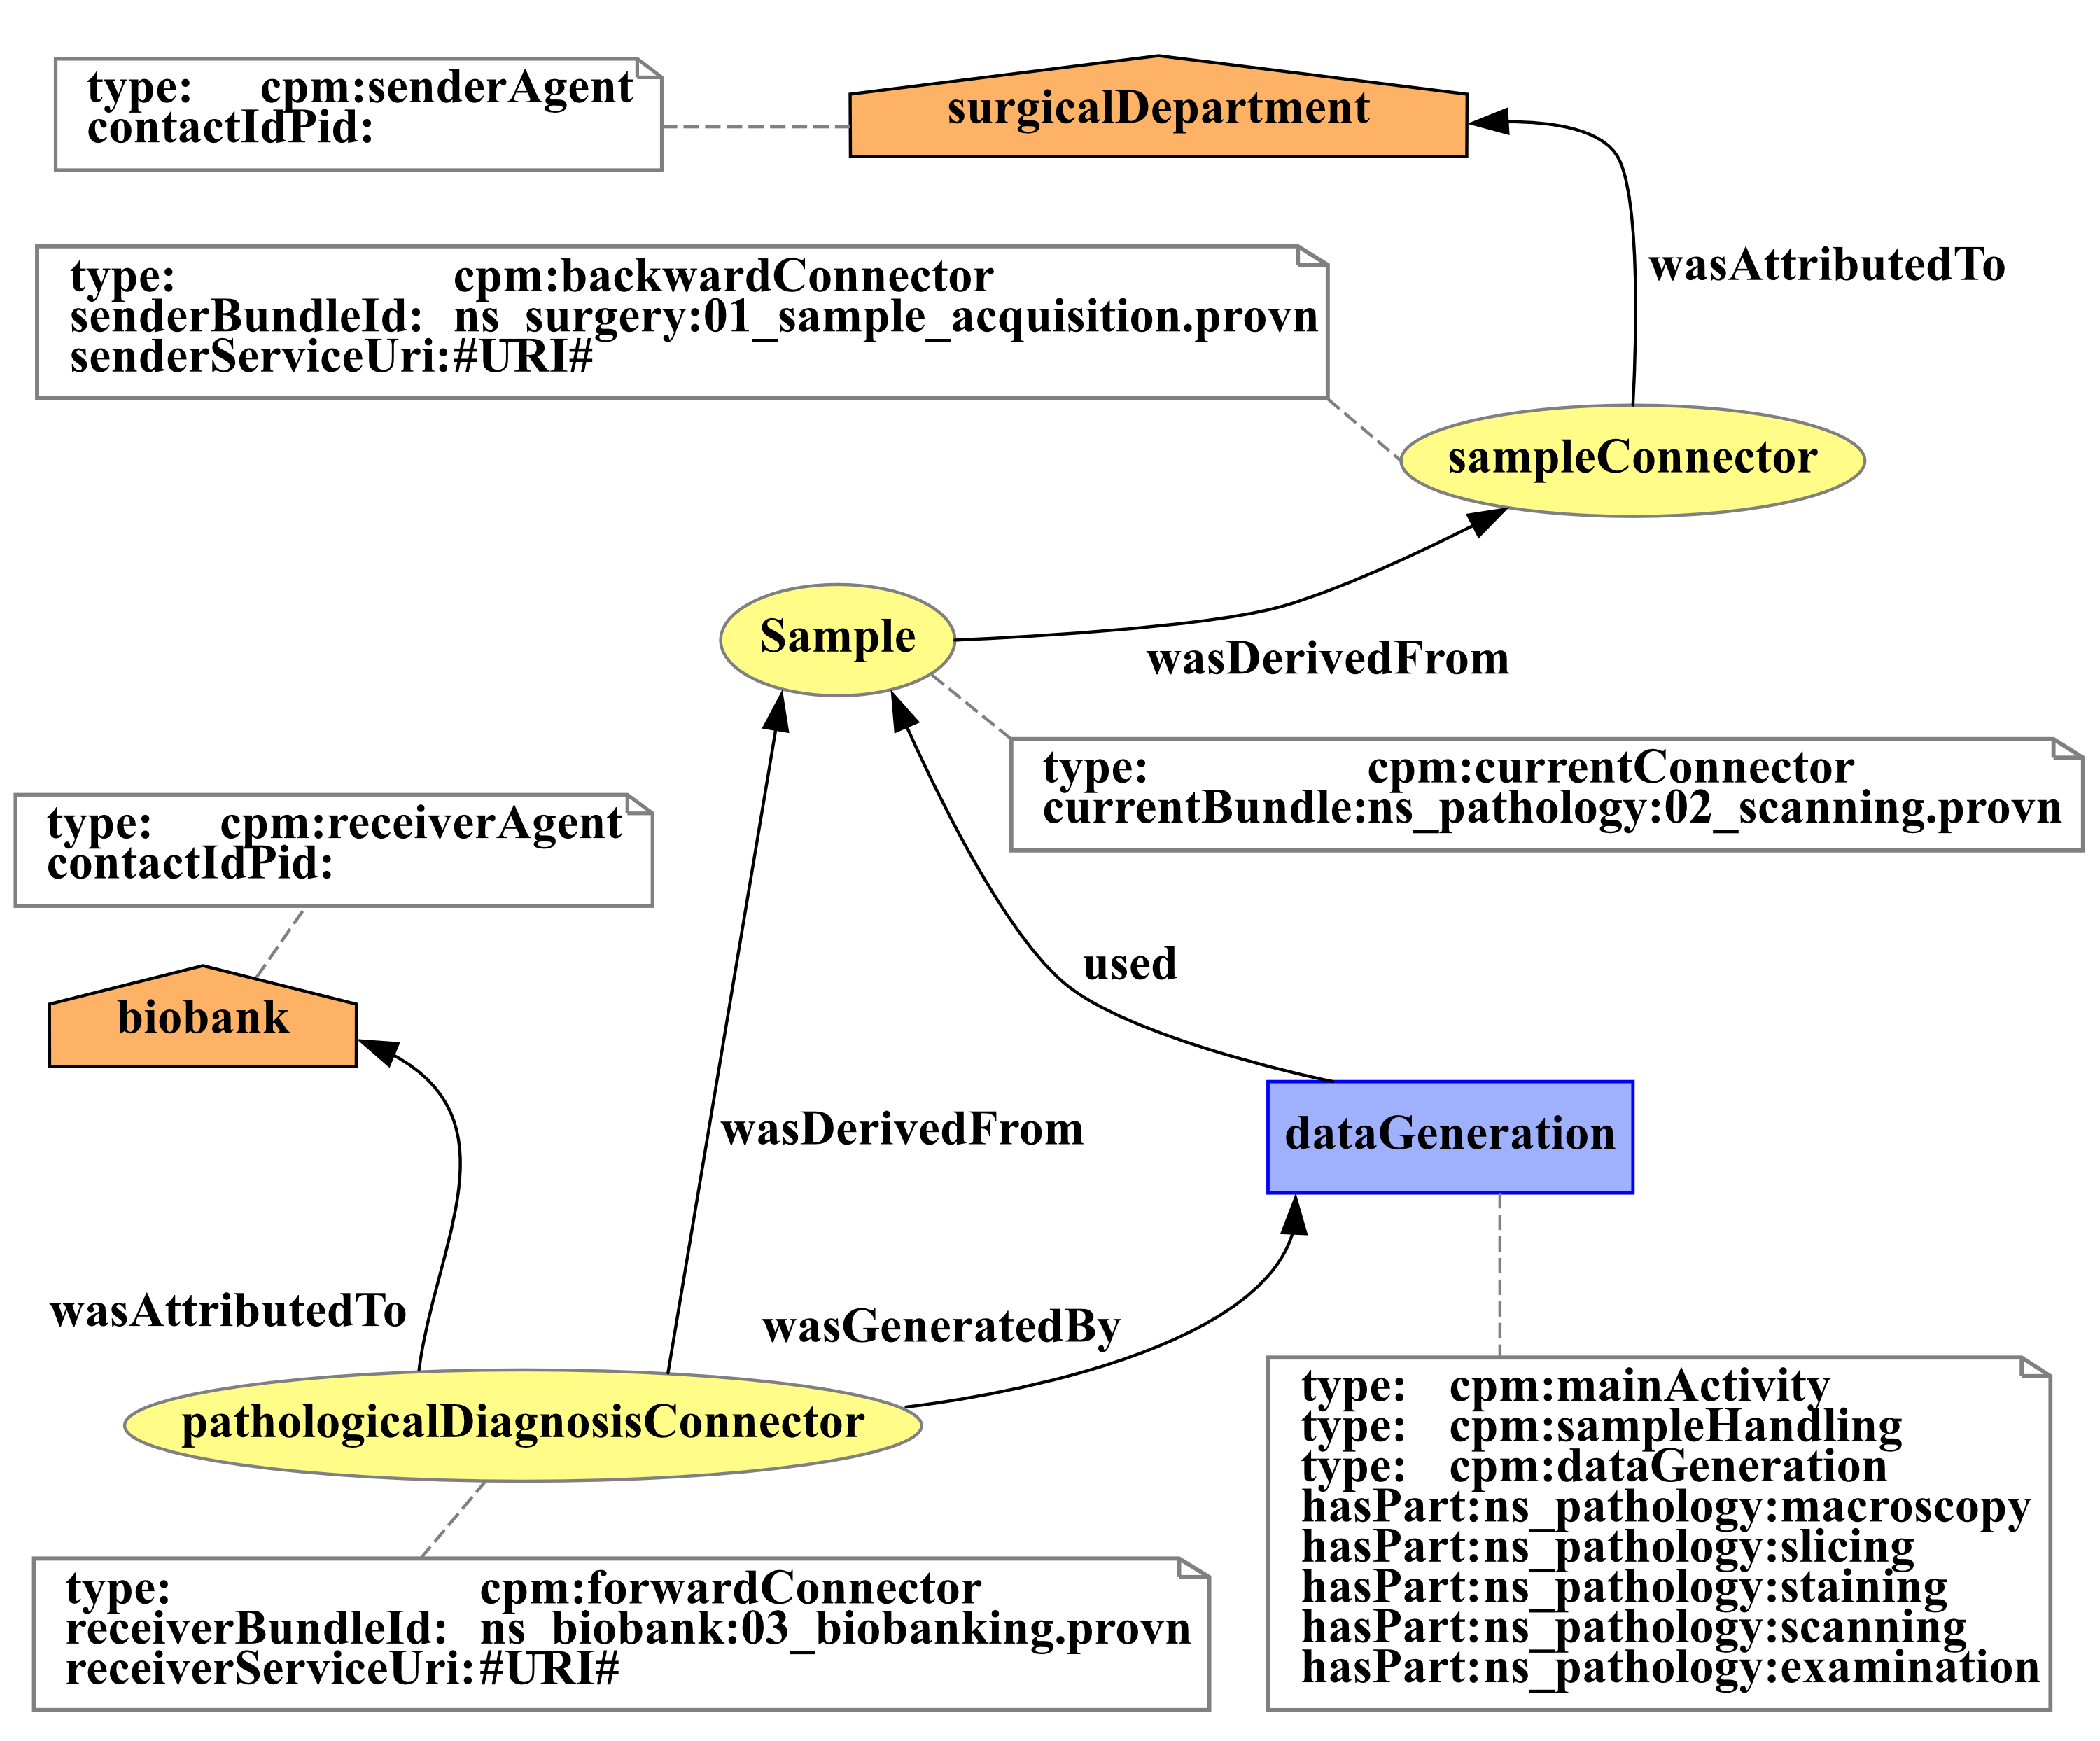
\includegraphics[width=9cm]{fithesis/images/examplebigger.png}
  \end{center}
  \caption{Excerpt from a PROV-N document}
  \label{fig:bundleexample4}
\end{figure}


\chapter{Implementation}
\section{Used technologies}
\shorthandoff{-}
\subsection{ProvToolBox}
Lorem ipsum dolor sit amet, consectetur adipiscing elit. Integer finibus commodo leo. Nullam blandit imperdiet magna, sit amet tempor tortor sagittis vitae. Lorem ipsum dolor sit amet, consectetur adipiscing elit. Cras elementum diam vel eros tristique, at maximus tortor ultricies.

\subsubsection{PROV MODEL}
Lorem ipsum dolor sit amet, consectetur adipiscing elit. Integer finibus commodo leo. Nullam blandit imperdiet magna, sit amet tempor tortor sagittis vitae. Lorem ipsum dolor sit amet, consectetur adipiscing elit. Cras elementum diam vel eros tristique, at maximus tortor ultricies.

\subsubsection{PROV INTEROP: LIGHT}
Lorem ipsum dolor sit amet, consectetur adipiscing elit. Integer finibus commodo leo. Nullam blandit imperdiet magna, sit amet tempor tortor sagittis vitae. Lorem ipsum dolor sit amet, consectetur adipiscing elit. Cras elementum diam vel eros tristique, at maximus tortor ultricies.

\subsection{Jackson Databind}
Lorem ipsum dolor sit amet, consectetur adipiscing elit. Integer finibus commodo leo. Nullam blandit imperdiet magna, sit amet tempor tortor sagittis vitae. Lorem ipsum dolor sit amet, consectetur adipiscing elit. Cras elementum diam vel eros tristique, at maximus tortor ultricies.

\subsection{GitLab4J API}
Lorem ipsum dolor sit amet, consectetur adipiscing elit. Integer finibus commodo leo. Nullam blandit imperdiet magna, sit amet tempor tortor sagittis vitae. Lorem ipsum dolor sit amet, consectetur adipiscing elit. Cras elementum diam vel eros tristique, at maximus tortor ultricies.

\subsection{JLine Bundle}
Lorem ipsum dolor sit amet, consectetur adipiscing elit. Integer finibus commodo leo. Nullam blandit imperdiet magna, sit amet tempor tortor sagittis vitae. Lorem ipsum dolor sit amet, consectetur adipiscing elit. Cras elementum diam vel eros tristique, at maximus tortor ultricies.

\subsection{Jansi}
Lorem ipsum dolor sit amet, consectetur adipiscing elit. Integer finibus commodo leo. Nullam blandit imperdiet magna, sit amet tempor tortor sagittis vitae. Lorem ipsum dolor sit amet, consectetur adipiscing elit. Cras elementum diam vel eros tristique, at maximus tortor ultricies.

\subsection{Apache Maven Shade Plugin}
Lorem ipsum dolor sit amet, consectetur adipiscing elit. Integer finibus commodo leo. Nullam blandit imperdiet magna, sit amet tempor tortor sagittis vitae. Lorem ipsum dolor sit amet, consectetur adipiscing elit. Cras elementum diam vel eros tristique, at maximus tortor ultricies.
\shorthandon{-}

\section{Runtime}
Lorem ipsum dolor sit amet, consectetur adipiscing elit. Integer finibus commodo leo. Nullam blandit imperdiet magna, sit amet tempor tortor sagittis vitae. Lorem ipsum dolor sit amet, consectetur adipiscing elit. Cras elementum diam vel eros tristique, at maximus tortor ultricies. Curabitur urna magna, dictum at porta rutrum, congue nec justo. Nam ac rhoncus lectus. Ut feugiat volutpat ornare. Mauris quis neque nec lorem vestibulum iaculis. Proin posuere nisi eget nisi tristique, eu tempus nibh ultricies.

\section{Problems during implementation}
Lorem ipsum dolor sit amet, consectetur adipiscing elit. Integer finibus commodo leo. Nullam blandit imperdiet magna, sit amet tempor tortor sagittis vitae. Lorem ipsum dolor sit amet, consectetur adipiscing elit. Cras elementum diam vel eros tristique, at maximus tortor ultricies.


\chapter{Manual}
\shorthandoff{-}
\section{Set-up}
To utilize the library, it is necessary to have Maven and Java properly configured. To simplify the process for users, the implementation is currently spread across multiple Git repositories, including two on FI and ICS GitLab sites and one on the author's personal GitHub page. To obtain the library, clone the repository or use the download button to retrieve the entire repository bundled in a zip or another archive file.

\subsection{Retrieving the repository}
In order to clone a repository, it is important to confirm that Git is installed on the device. Following this, proceed to the repository's page on GitLab or GitHub and locate the "Clone" button. A URL to copy will be generated by clicking on this button. Next, launch the terminal or command prompt, navigate to the directory where the repository should be stored, and execute the command 'git clone [URL]', replacing [URL] with the URL you copied earlier. Doing this will generate a local copy of the repository on the device. If cloning is not possible, an alternative is to download the repository as a ZIP file. On the repository's page, look for the "Download ZIP" option, typically found in the same section as the clone option. Clicking on this will download the repository's contents in a compressed file, which can then be extracted to the preferred location.

\subsection{Simulating the environment}
The initiation of simulation files is the first step in simulating an environment, which requires the retrieval of specific files necessary for the simulated environment to function effectively. To achieve this, the cloned repository should be opened in the console. The submodule can be navigated by using the command.

\begin{verbatim}
$ cd. \src\main\resources\bthesis-provenancechain-digpat  
\end{verbatim}

Once the submodule is reached, the command 

\begin{verbatim}
$ git submodule foreach git fetch –tags
\end{verbatim}

should be executed. After it finishes, there should be no output. Finally, the command

\begin{verbatim}
$ git submodule update --init --recursive  
\end{verbatim}

should be run to conclude the process. This will ensure that the bthesis-provenancechain-digpat submodule contains the required .provn files.

\section{Building}
The jar file is packaged using the Maven Shade plugin, which is the preferred method. To create the jar file, navigate to the cloned repository using the console and run the \textbf{\texttt{'mvn clean package'}} command. After creating the jar file, it can be launched by executing the command \textbf{\texttt{'java -jar }\path{.\target\BThesis-ProvenanceChain-VERSION-shaded.jar'}}. In the event that the intended environment does not have a JRE, the \textbf{\texttt{'jpackage'}} command line tool provided by Java can be used to create a platform-specific installer.

\section{Omitting the simulated environment}
To facilitate traversal simulation, the implementation employs several classes and files that provide the necessary objects for the algorithm to function. These classes have been transferred to packages labeled 'bthesis.provenancechain.simulation' and 'bthesis.metageneration' to enhance clarity. At the same time, the required files reside in the previously mentioned submodule 'src.main.resources.bthesis-provenancechain-digpat'. However, these components can be omitted if the required classes are adequately substituted.
\shorthandon{-}


\chapter*{Conclusion}
\markright{\textsc{Conclusion}}
\addcontentsline{toc}{chapter}{Conclusion}
\shorthandoff{-}
Lorem ipsum dolor sit amet, consectetur adipiscing elit. Integer finibus commodo leo. Nullam blandit imperdiet magna, sit amet tempor tortor sagittis vitae. Lorem ipsum dolor sit amet, consectetur adipiscing elit. Cras elementum diam vel eros tristique, at maximus tortor ultricies. Curabitur urna magna, dictum at porta rutrum, congue nec justo. Nam ac rhoncus lectus. Ut feugiat volutpat ornare. Mauris quis neque nec lorem vestibulum iaculis. Proin posuere nisi eget nisi tristique, eu tempus nibh ultricies.
\shorthandon{-}

After linking a bibliography data\-base files to the document using
the \verb"\"\texttt{thesis\discretionary{-}{}{}setup\{bib\discretionary{=}{=}{=}%
\{\textit{file1},\textit{file2},\,\ldots\,\}\}} command, you can
start citing the entries. This is just dummy text
\parencite{borgman03} lightly sprinkled with citations
\parencite[p.~123]{greenberg98}. Several sources can be cited at
once: \cite{borgman03,greenberg98,thanh01}.
\citetitle{greenberg98} was written by \citeauthor{greenberg98} in
\citeyear{greenberg98}. We can also produce \textcite{greenberg98}%
\ or %% Let us define a compound command:
\def\citeauthoryear#1{(\textcite{#1},~\citeyear{#1})}%
\citeauthoryear{greenberg98}%
. The full bibliographic citation is:
\emph{\fullcite{greenberg98}}. We can easily insert a bibliographic
citation into the footnote\footfullcite{greenberg98}.

\printbibliography[heading=bibintoc]

\end{document}
